\documentclass[a4paper,11pt]{article}

\usepackage{listings}
\usepackage{framed}


\usepackage{CJKutf8}
\usepackage{graphicx}
\usepackage{fancyhdr}
\usepackage{cite}
\usepackage{amsmath}
\usepackage[framed,numbered,autolinebreaks,useliterate]{mcode}
\usepackage{booktabs}
\usepackage{indentfirst}
\setlength{\parindent}{0em}
\usepackage{setspace}
\usepackage{subfigure}
\usepackage{float}
\usepackage{booktabs}
\usepackage{geometry}
\renewcommand{\dblfloatpagefraction}{.9}
\geometry{a4paper,scale=0.8}
\begin{document}
\begin{spacing}{1.2}
\begin{CJK}{UTF8}{gbsn}
\title{基于Python实现的多协议首部检验}
\author{软件2003杜睿}
\date{}
\maketitle{}

\abstract{\textbf{设计内容}}
在网络数据传输过程中,网络上的数据都要通过差错控制来保证其数据的正确性。进行差错检测和控制的主要方法是:发送放在需要发送的数据后面增加一定的冗余信息,这些冗余信息通常是通过对发送的数据进行某种算法计算而得到的。接收方对数据进行同样的计算然后比较冗余信息以检测数据是否正确。输入IP、TCP和UDP等数据包,能给出该数据包首部检验和检验的过程,判断首部数据包是否有差错。

\section{需求分析}

根据题目所述,需要设计一个程序来检查网络数据包是否存在差错。从大体功能的角度说,需要设计以下模块:

\begin{description}
	\item [数据包解析模块] 解析数据包,提取字段,并将其传递给校验和计算模块;
	\item [校验和计算模块] 计算校验和,检查数据包是否存在差错;
	\item [界面与交互模块] 告知用户数据包的首部是否存在差错,并展现详细的计算过程。
\end{description}


为确保程序能够正确地解析和计算不同类型的数据包,在实现这些模块时,还需要考虑不同协议的字段长度、伪首部的自动化生成问题。

\section{概要设计}

根据TCP/IP体系结构,数据的解析和校验应当是分层的。

\begin{figure}[htbp]
    \centering
    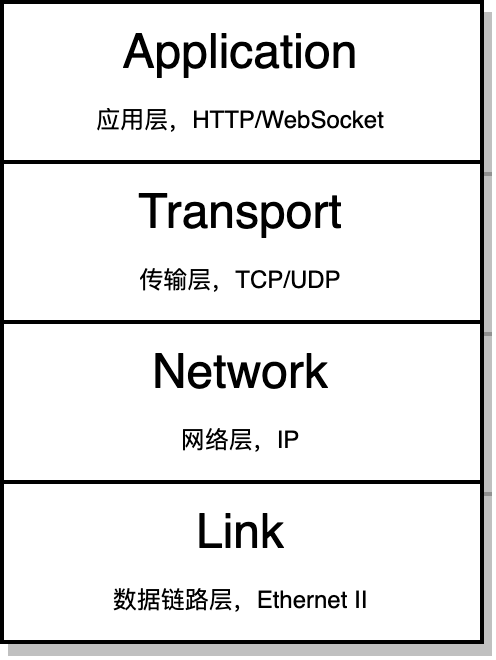
\includegraphics[scale=1.4]{i-4.png}
    \caption{TCP/IP的体系结构}
\end{figure}

\newpage

\begin{figure}[htbp]
    \centering
    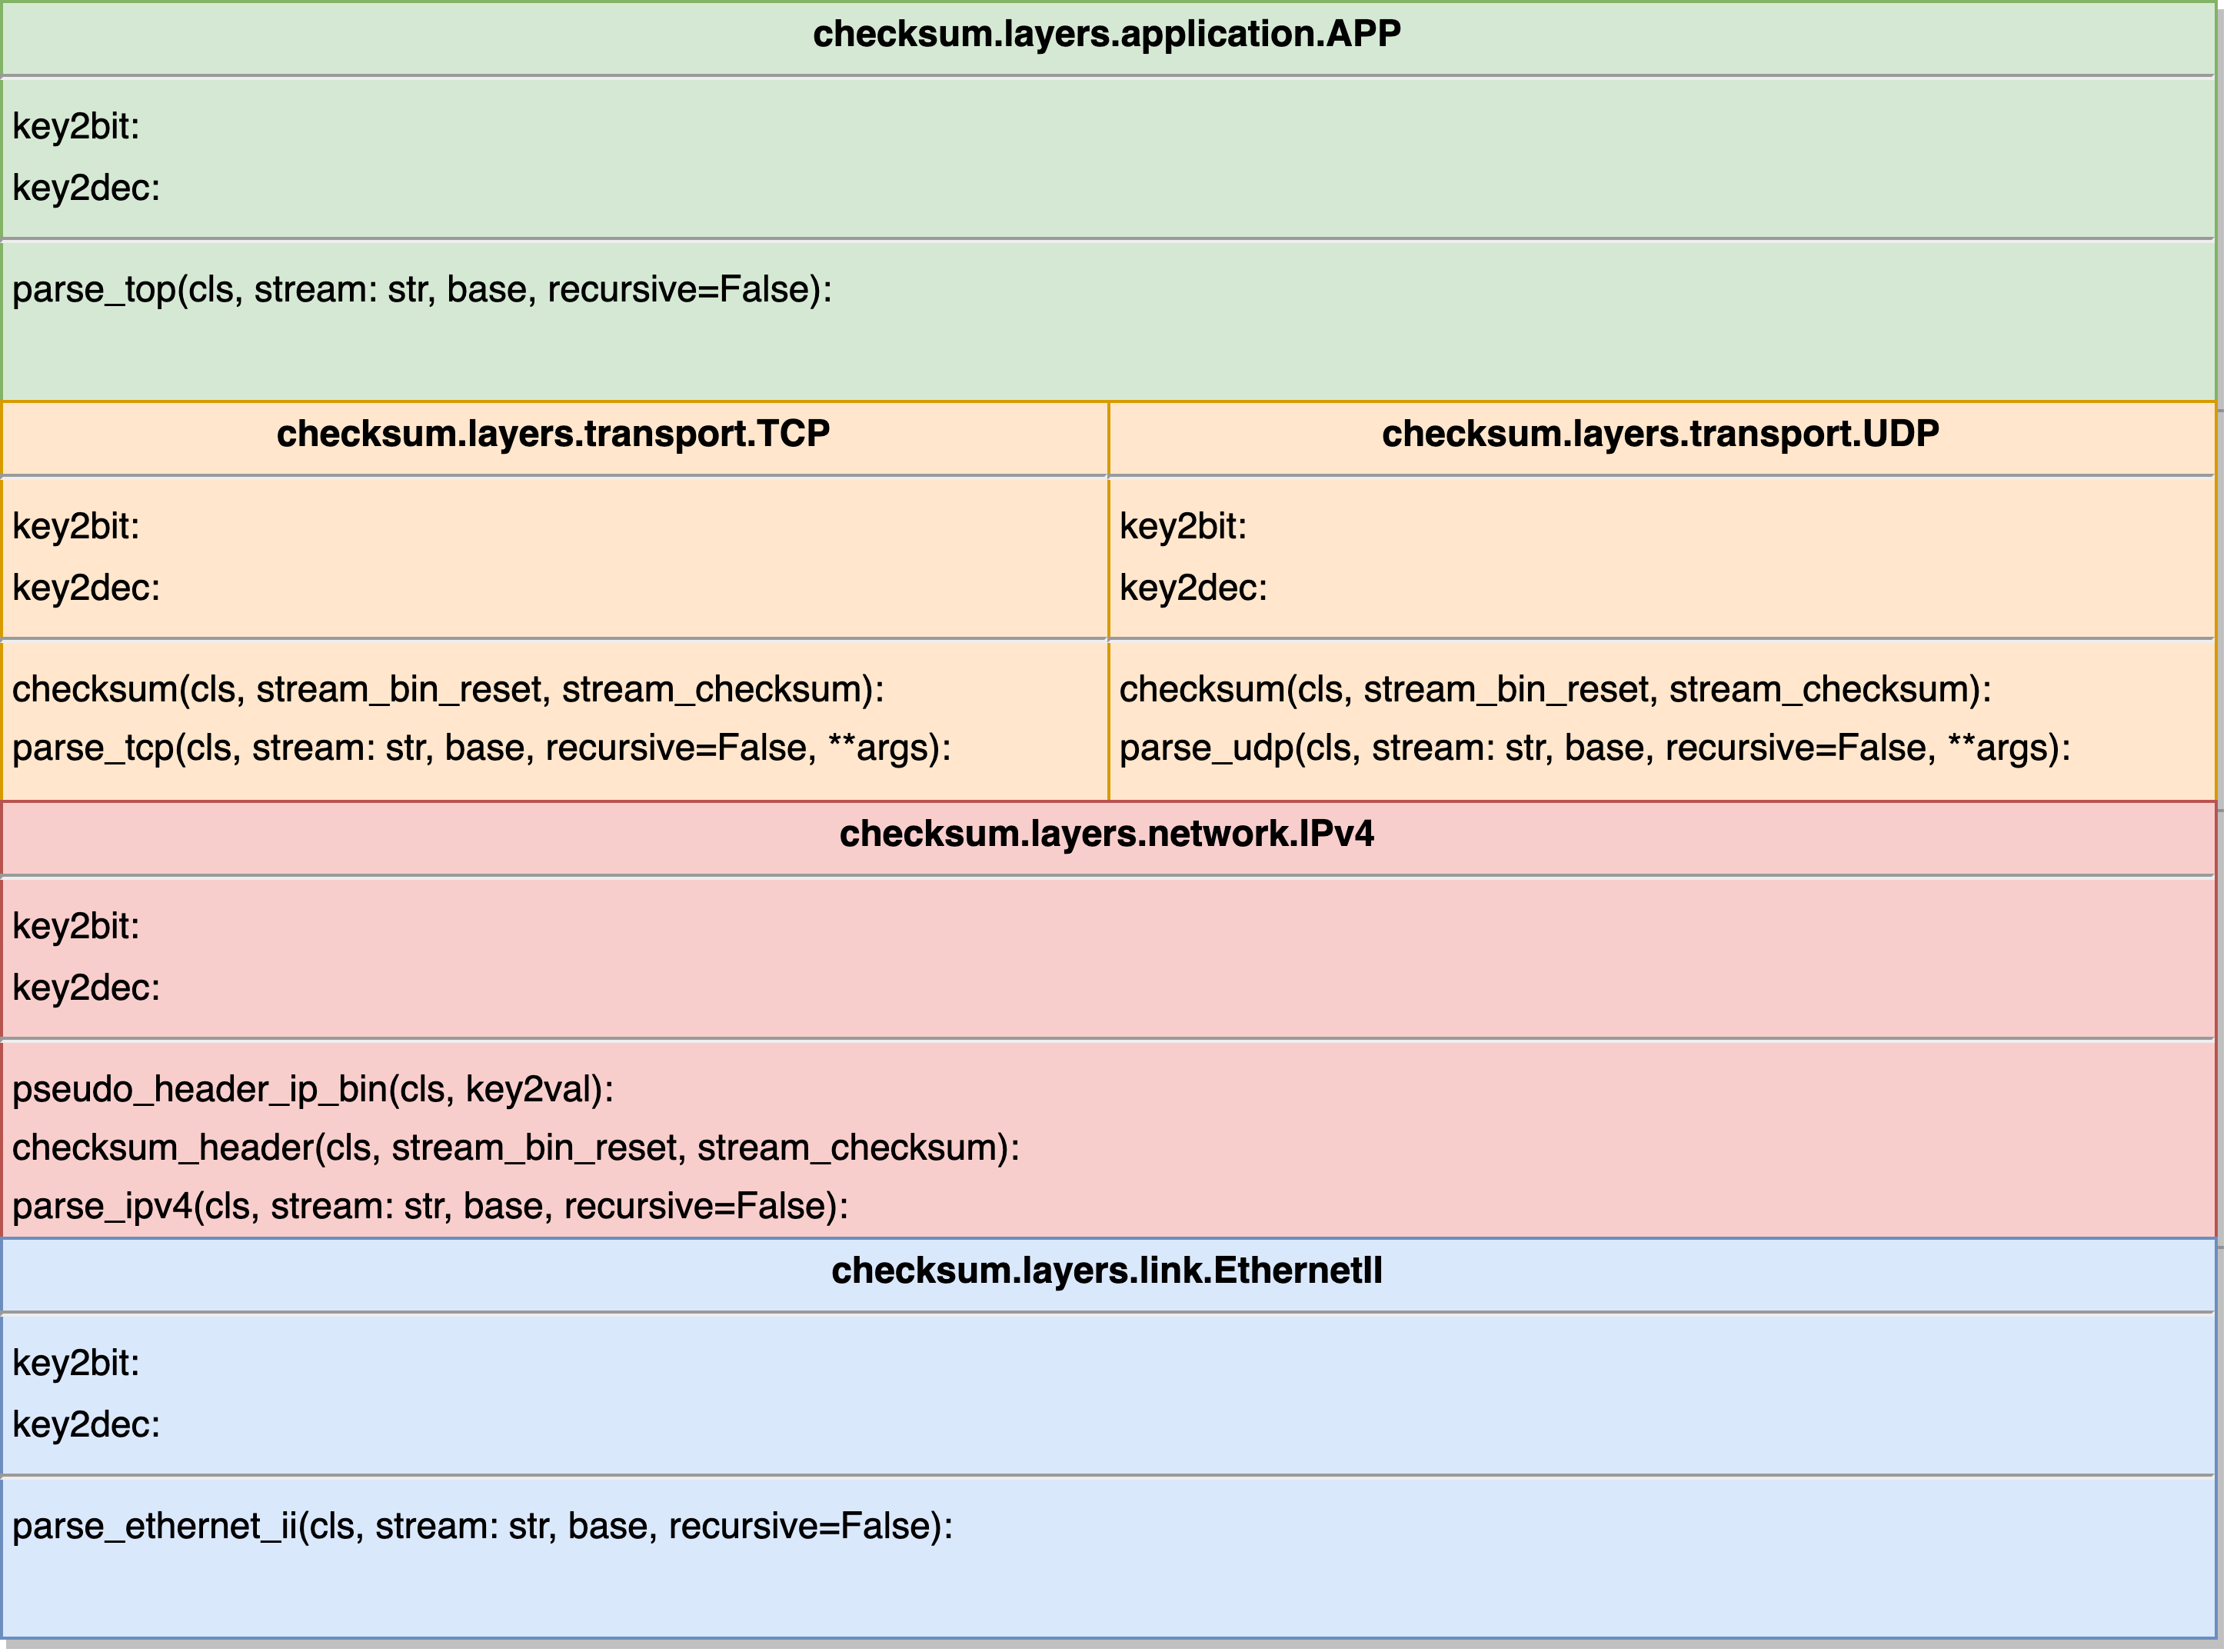
\includegraphics[height=20.4em]{i-class.png}
    \caption{基于体系结构设计的各层}
\end{figure}

\begin{description}
	\item [key2bit] \{字段, 比特长度\},例如,\{"mac\_addr\_dst", 6*8\}。
	\item [key2dec] \{字段,解析函数\},例如,\{"type\_ethernet", type\_ethernet(stream\_hex)\}。
	\item [parser] 静态函数,输入数据流、对应进制,输出解析结果、校验位置零的比特流。
\end{description}


\begin{figure}[htbp]
    \centering
    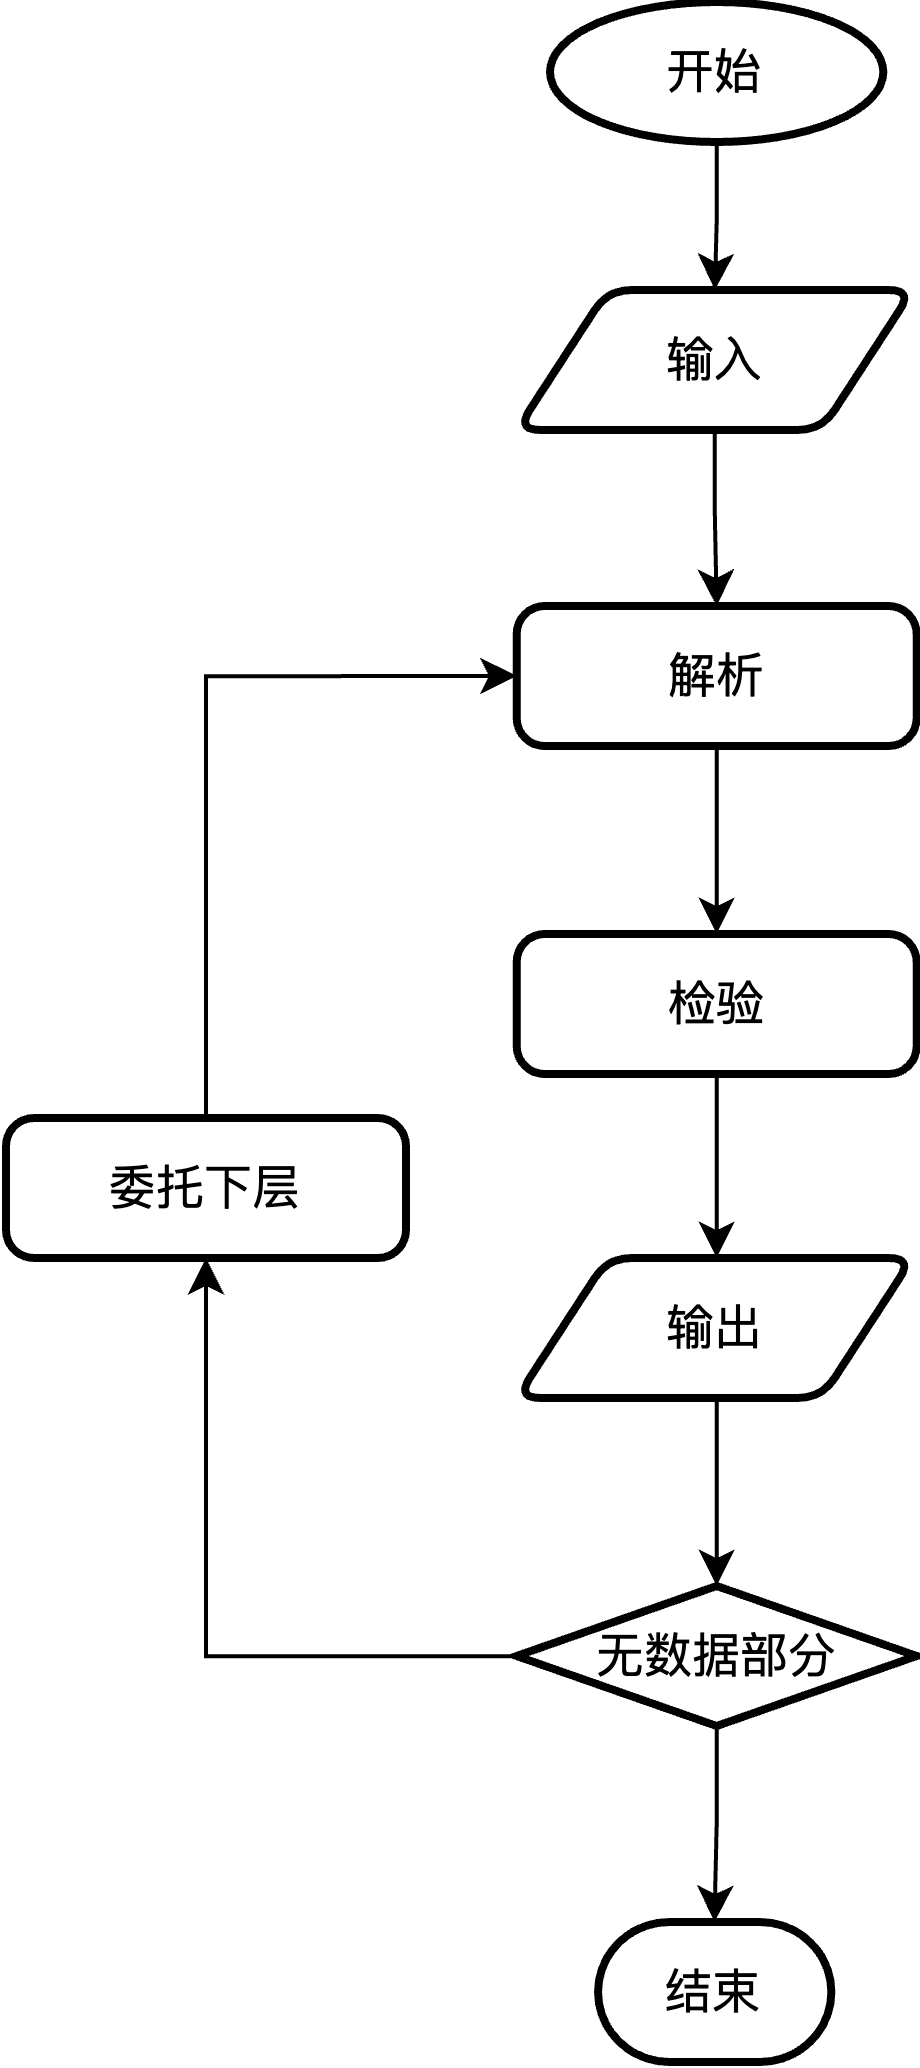
\includegraphics[height=21em]{i-proc.png}
    \caption{各层解析流程}
\end{figure}

每一层的执行流程是,利用\textbf{key2bit}和\textbf{key2dec}获悉各个字段的比特长度,经过进制转换、添零补丁,对进制流串进行分割,并用键值对存储解析结果,然后执行检验过程。对于传输层的检验而言,需要网络层传递伪首部。

\newpage

\subsection{解析器}

\begin{description}
	\item [输入] 网络数据包
	\item [输出] 数据包各字段的值
	\item [设计] 根据数据包的协议类型,确定该数据包的首部格式以及各字段的位置和长度。读取数据包中的各个字段,将它们存储到一个数据结构中,该数据结构可以使用一个字典来表示,以便能够方便地访问各个字段的值。
\end{description}

\begin{figure}[h]
    \centering
    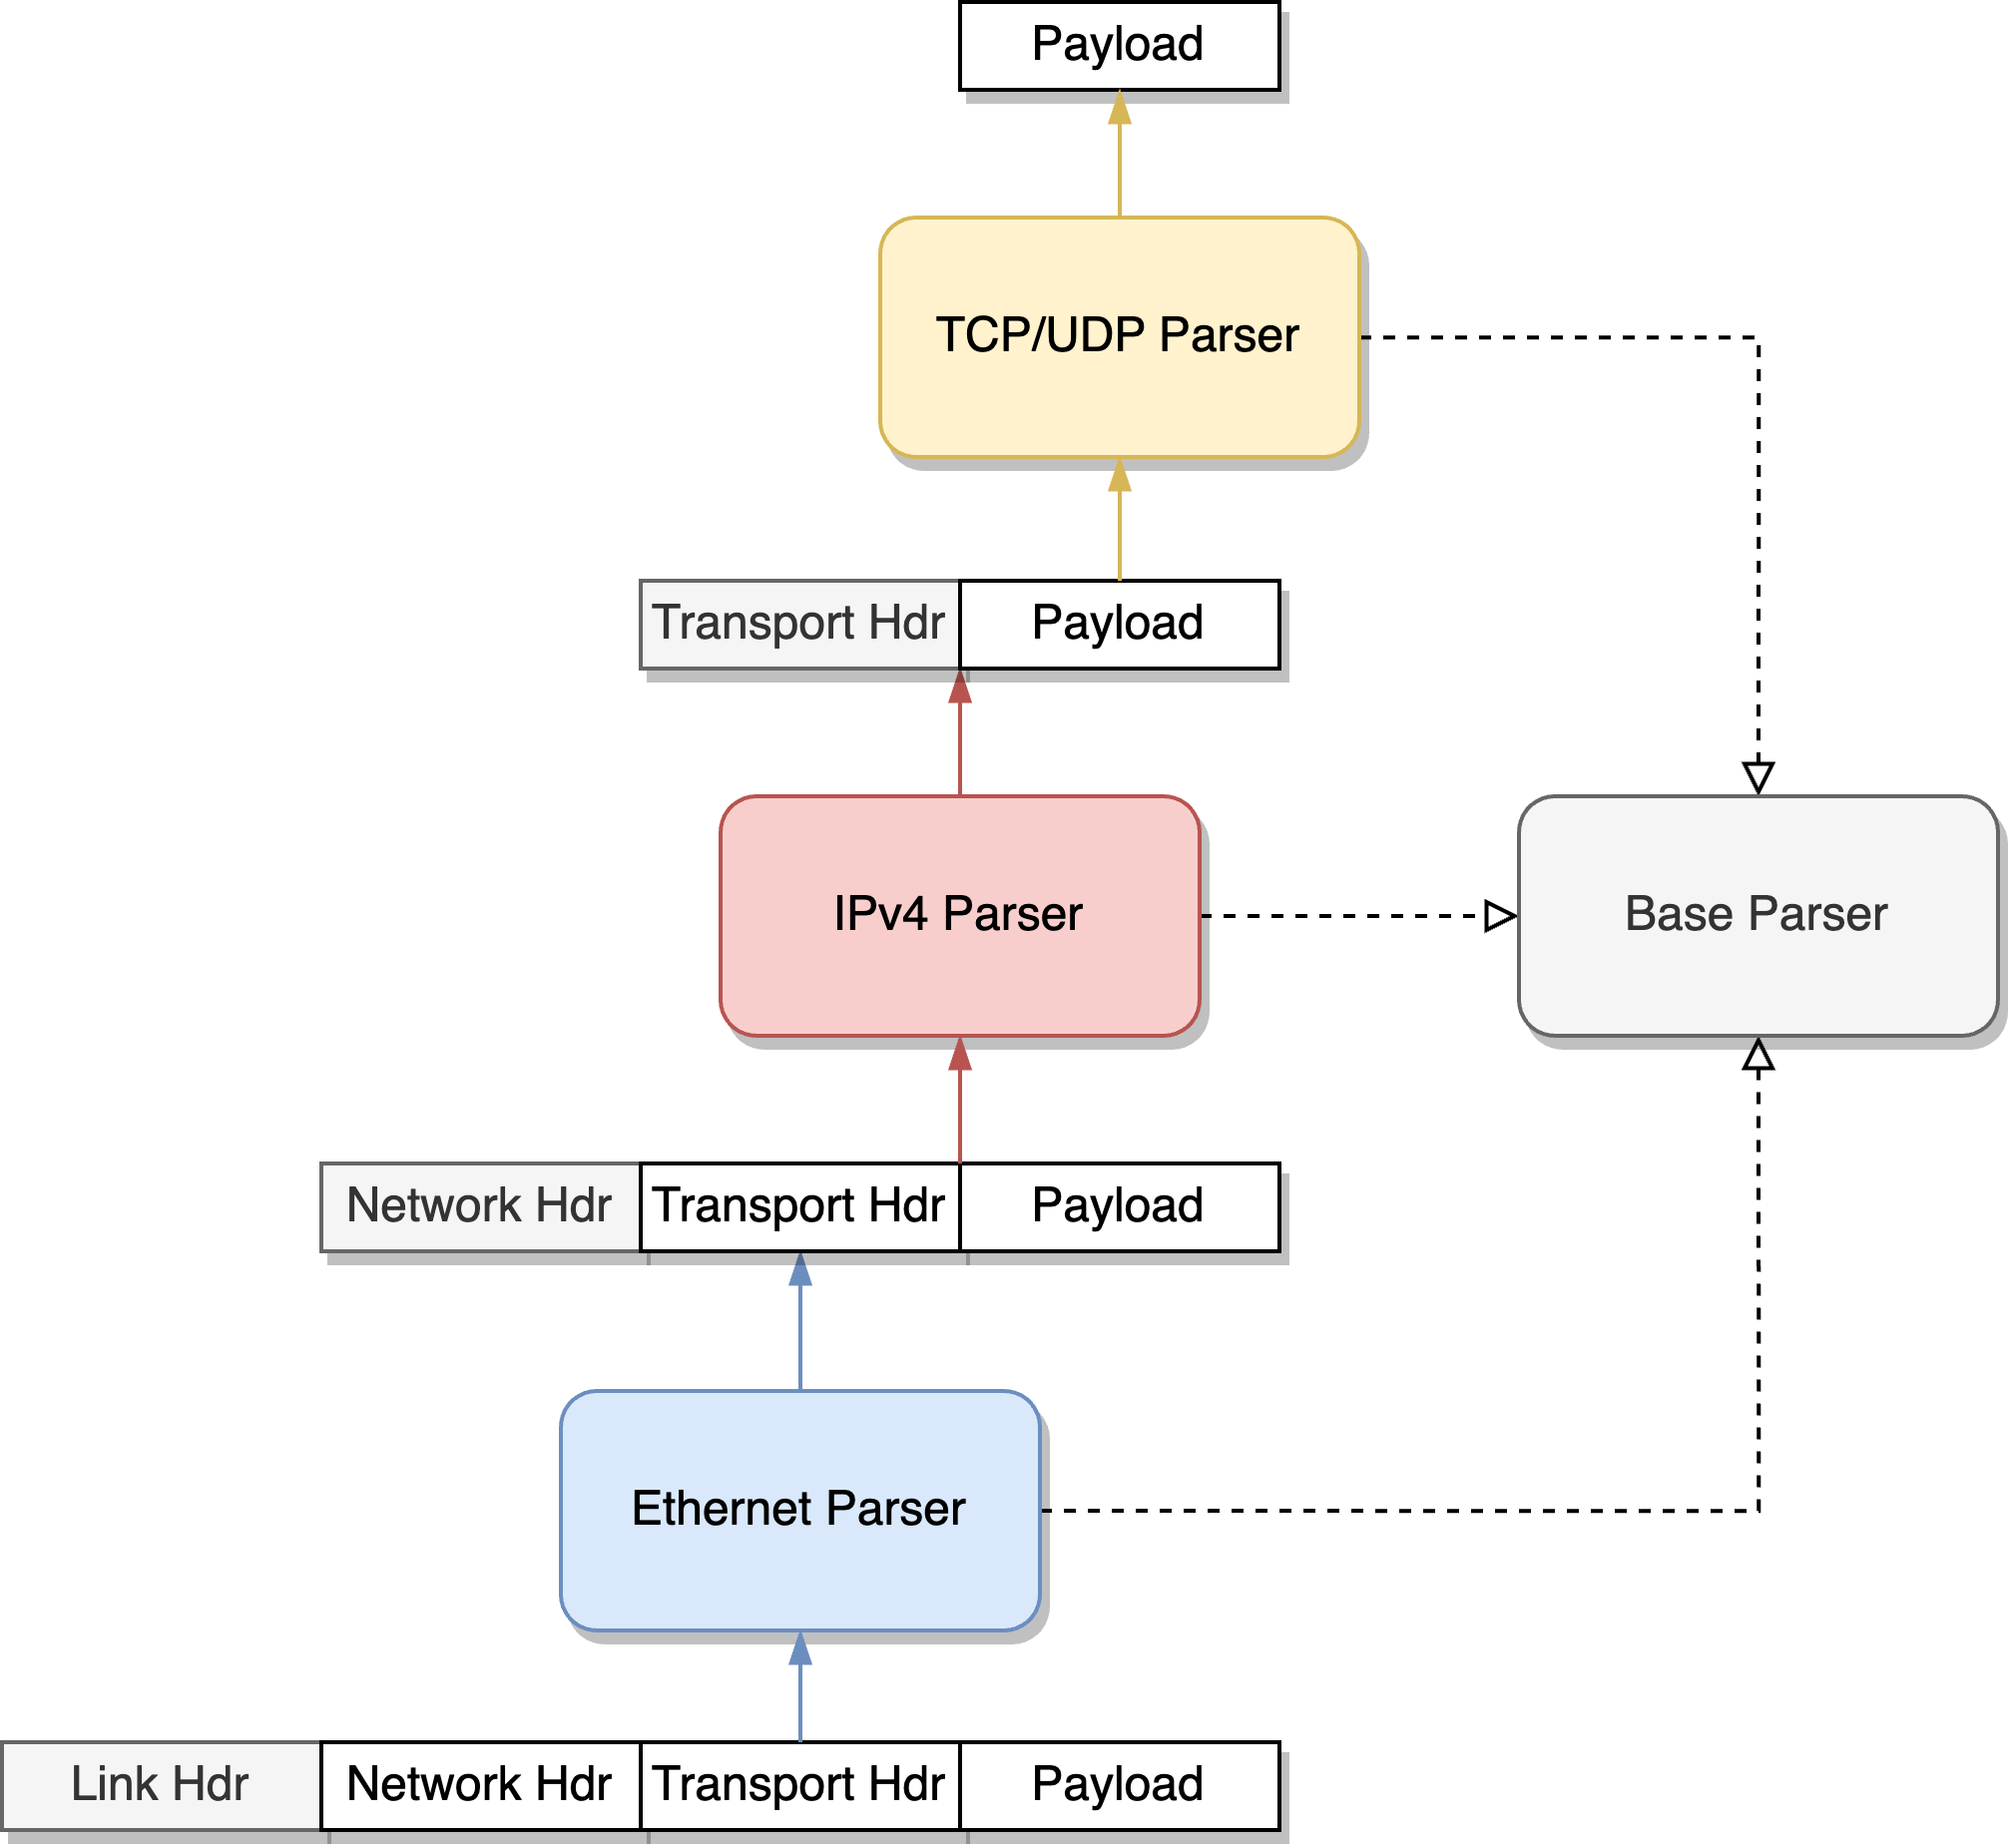
\includegraphics[scale=0.6]{i-par.png}
    \caption{数据包的分层解析}
\end{figure}

\subsection{校验器}

\begin{description}
	\item [输入] 待校验的数据流、检验和
	\item [输出] 校验和计算结果
	\item [设计] (待检验的数据流需要各层进行修饰)累加,回卷,加上校验和,为“0xFFFF”即正确。
\end{description}

\begin{figure}[h]
    \centering
    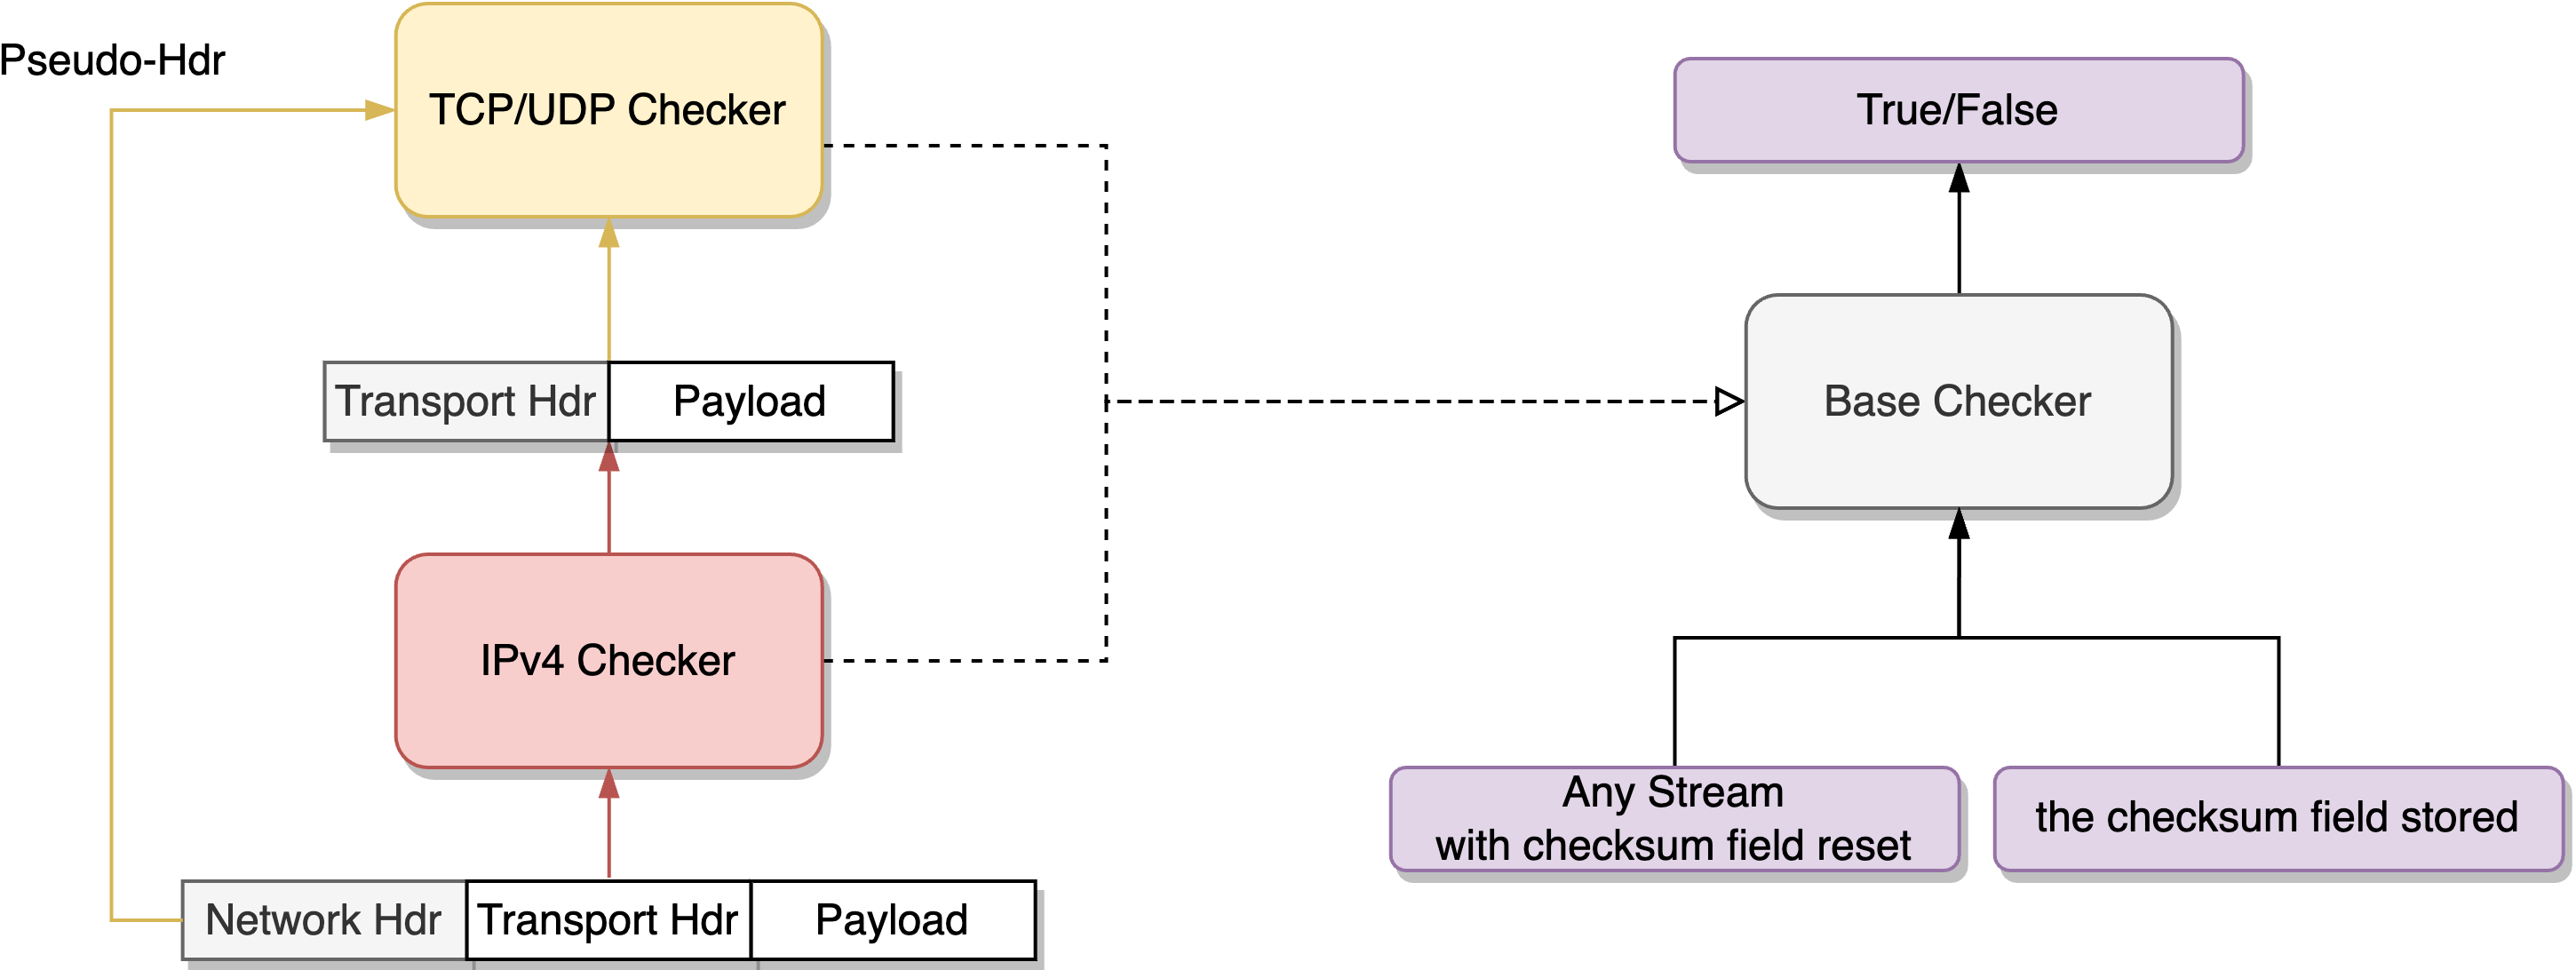
\includegraphics[scale=0.6]{i-check.png}
    \caption{数据包的分层校验}
\end{figure}





\section{编码实现}

\subsection{对各层的实现\footnote{本程序支持数据链路层作为输入,此处仅展示网络层和传输层}}

\begin{description}
	\item [程序输入] 2进制或16进制
	\item [解析器] 按2进制切分,16进制存储(展示),同步返回置零后的2进制流
	\item [校验器] 默认输入(2进制数据流、16进制校验和),按16进制计算(加和\footnote{加和使用10进制}、回卷)
\end{description}

\subsubsection{网络层}

\begin{lstlisting}[language = Python, numbers=left, numberstyle=\tiny,keywordstyle=\color{blue!70},commentstyle=\color{red!50!green!50!blue!50},frame=shadowbox,rulesepcolor=\color{red!20!green!20!blue!20},basicstyle=\ttfamily]
"""
the THIN WAIST's JOB:

1. deliver packets end-to-end across the Internet, from the SOURCE end to the eventual DESTINATION end.
2. no promises and no guarantees
"""
from checksum import dataset, process_dataset
from checksum.layers.transport import TCP, UDP
from checksum.utils import parser, decoder, checker
from checksum.utils.decoder import type_protocol
from checksum.utils.formatter import nip_prefix
from checksum.utils.static import String
from checksum.utils.rich_console import console


class IPv4:
    key2bit = {
        String.ip_version: 4,
        String.length_header: 4,
        String.type_service: 8,
        String.length_total_packet: 16,
        String.id_packet: 16,
        String.flags: 3,
        String.offset_fragment: 13,
        String.time_to_live: 8,
        String.id_protocol: 8,
        String.checksum: 16,
        String.ip_addr_src: 32,
        String.ip_addr_dst: 32,
        String.data_payload: -1,
    }

    key2dec = {
        String.id_protocol: type_protocol
    }

    @classmethod
    def pseudo_header_ip_bin(cls, key2val):
        ip_addr_src = nip_prefix(bin(int(key2val[String.ip_addr_src], 16)), 2).zfill(4 * 8)
        ip_addr_dst = nip_prefix(bin(int(key2val[String.ip_addr_dst], 16)), 2).zfill(4 * 8)
        id_protocol = nip_prefix(bin(int(key2val[String.id_protocol], 16)), 2).zfill(2 * 8)
        return ip_addr_src + ip_addr_dst + id_protocol

    @classmethod
    def checksum_header(cls, stream_bin_reset, stream_checksum):
        process_dataset['network'] = checker.check(nip_prefix(stream_bin_reset)[:160], stream_checksum, base=2,
                                                   pseudo=False)

    @classmethod
    def parse_ipv4(cls, stream: str, base, recursive=False):
        assert stream != "" and stream is not None, "NULL STREAM"

        console.rule("[bold green] network layer parsing [/bold green]")

        key2val, stream_bin_reset = parser.parse(cls.key2bit, stream, base)
        key2exp = decoder.decode(cls.key2bit, key2val, cls.key2dec)

        for key in key2exp.keys():
            if key in cls.key2dec.keys():
                console.print(f"{key} : [bold red italic]{key2exp[key]}[/bold red italic]")
            else:
                console.print(f"{key} : [black]{key2exp[key]}[/black]")

        dataset['network'] = key2exp

        cls.checksum_header(stream_bin_reset, key2val[String.checksum])

        if recursive:
            if key2val[String.data_payload] is not None:
                if key2exp[String.id_protocol] == String.tcp:
                    TCP.parse_tcp(key2val[String.data_payload], 16, recursive, pseudo=cls.pseudo_header_ip_bin(key2val))
                elif key2exp[String.id_protocol] == String.udp:
                    UDP.parse_udp(key2val[String.data_payload], 16, recursive, pseudo=cls.pseudo_header_ip_bin(key2val))
                else:
                    assert False, "Transport Protocol Not Supported"
        else:
            console.rule("[bold green]EOF[/bold green]")


# https://www.cnblogs.com/jersey/archive/2011/11/29/2267492.html
class IPv6:
    key2bit = {
        String.ip_version: 4,
        String.type_service: 8,
        String.label_flow: 20,
        String.length_payload: 6,
        String.header_next: 8,
        String.limit_hop: 8,
        String.ip_addr_src: 128,
        String.ip_addr_dst: 128,
        String.data_payload: -1,
    }

    key2dec = {
        String.class_traffic: type_protocol
    }

    @classmethod
    def parse_ipv6(cls, param, param1, recursive):
        pass

         
\end{lstlisting}

\subsubsection{传输层}



\begin{lstlisting}[language = Python, numbers=left, numberstyle=\tiny,keywordstyle=\color{blue!70},commentstyle=\color{red!50!green!50!blue!50},frame=shadowbox,rulesepcolor=\color{red!20!green!20!blue!20},basicstyle=\ttfamily]
"""

TCP's JOB:

correctly delivered, with any lost/corrupted bank automatically retransmitted if needed
"""
from checksum import dataset, process_dataset
from checksum.layers.application import APP
from checksum.utils.rich_console import console
from checksum.utils import parser, decoder, checker
from checksum.utils.formatter import nip_prefix
from checksum.utils.static import String


class TCP:
    key2bit = {
        String.port_src: 16,
        String.port_dst: 16,
        String.sequence_first_byte: 32,
        String.sequence_acknowledgement: 32,
        String.length_header: 4,
        String.reserved: 6,
        String.flags: 6,
        String.size_window: 16,
        String.checksum: 16,
        String.pointer_urgent: 16,
        String.data_payload: -1
    }

    key2dec = {

    }

    @classmethod
    def checksum(cls, stream_bin_reset, stream_checksum):
        process_dataset['transport'] = checker.check(stream_bin_reset, stream_checksum, base=2)

    @classmethod
    def parse_tcp(cls, stream: str, base, recursive=False, **args):
        assert stream != "" and stream is not None, "NULL STREAM"

        console.rule("[bold green] transport layer parsing [/bold green]")

        key2val, stream_bin_reset = parser.parse(cls.key2bit, stream, base)
        key2exp = decoder.decode(cls.key2bit, key2val, cls.key2dec)

        for key in key2exp.keys():
            if key in cls.key2dec.keys():
                console.print(f"{key} : [bold red italic]{key2exp[key]}[/bold red italic]")
            else:
                console.print(f"{key} : [black]{key2exp[key]}[/black]")

        dataset['transport'] = key2exp

        data = stream_bin_reset[160:]

        # note the unit is byte
        stream_bin_reset = args.get("pseudo") \
                           + nip_prefix(bin(len(stream_bin_reset) // 8), 2).zfill(2 * 8) \
                           + nip_prefix(stream_bin_reset, 2)

        if len(data) % 16 != 0:
            stream_bin_reset = stream_bin_reset + "00000000"

        cls.checksum(stream_bin_reset, key2val[String.checksum])

        if key2val[String.data_payload] is None:
            recursive = False

        if recursive:
            APP.parse_top(key2val[String.data_payload], 16, recursive)
        else:
            console.rule("[bold green]EOF[/bold green]")


class UDP:
    key2bit = {
        String.port_src: 16,
        String.port_dst: 16,
        String.length_total_packet: 16,
        String.checksum: 16,
        String.data_payload: -1,
    }

    key2dec = {
    }

    @classmethod
    def checksum(cls, stream_bin_reset, stream_checksum):
        process_dataset['transport'] = checker.check(stream_bin_reset, stream_checksum, base=2)

    @classmethod
    def parse_udp(cls, stream: str, base, recursive=False, **args):
        assert stream != "" and stream is not None, "NULL STREAM"

        console.rule("[bold green] transport layer parsing [/bold green]")

        key2val, stream_bin_reset = parser.parse(cls.key2bit, stream, base)
        key2exp = decoder.decode(cls.key2bit, key2val, cls.key2dec)

        for key in key2exp.keys():
            if key in cls.key2dec.keys():
                console.print(f"{key} : [bold red italic]{key2exp[key]}[/bold red italic]")
            else:
                console.print(f"{key} : [black]{key2exp[key]}[/black]")

        dataset['transport'] = key2exp

        data = stream_bin_reset[64:]
        
        # differring from udp, the length field is not calculated
        stream_bin_reset = args.get("pseudo") \
                           + nip_prefix(bin(int(key2val[String.length_total_packet], 16)), 2).zfill(2 * 8) \
                           + nip_prefix(stream_bin_reset, 2)

        if len(data) % 16 != 0:
            stream_bin_reset = stream_bin_reset + "00000000"

        cls.checksum(stream_bin_reset, key2val[String.checksum])

        if key2val[String.data_payload] is None:
            recursive = False

        if recursive:
            APP.parse_top(key2val[String.data_payload], 16)
        else:
            console.rule("[bold green]EOF[/bold green]")

	
\end{lstlisting}

\subsection{对校验的实现}

\begin{lstlisting}[language = Python, numbers=left, numberstyle=\tiny,keywordstyle=\color{blue!70},commentstyle=\color{red!50!green!50!blue!50},frame=shadowbox,rulesepcolor=\color{red!20!green!20!blue!20},basicstyle=\ttfamily]
from checksum import Data
from checksum.utils.rich_console import console
from checksum.utils.formatter import nip_prefix, print_hex, bin2hex


# https://blog.csdn.net/whatday/article/details/104051481
def complement(n4: str):
    n4 = nip_prefix(n4).zfill(4)
    n4 = list(n4)
    for i in range(len(n4)):
        n4[i] = nip_prefix(hex(15 - int(n4[i], 16)))
    return hex(int(''.join(n4), 16))


# https://www.bilibili.com/video/BV1fD4y1q7Dj
def double_sum(stream_hex: str):
    stream_hex = nip_prefix(stream_hex)
    # FIXME
    l = int(stream_hex[-4:], 16)
    r = int(stream_hex[:-4], 16)
    return l + r


def check(stream_hex: str, stream_checksum: str, base=16, pseudo=True):
    if base == 2:
        stream_hex = bin2hex(stream_hex)

    stream_hex, stream_checksum = map(nip_prefix, (stream_hex, stream_checksum))

    process = {Data.pseudo: pseudo,
               Data.reset: print_hex(stream_hex),
               Data.detail: [],
               Data.double_sum: [],
               Data.complement: [],
               Data.result: False}

    _sum = 0
    _tmp = 0
    for i in range(4, len(stream_hex) + 1, 4):
        _tmp += int(stream_hex[i - 4:i], 16)
        process[Data.detail].append(
            f"{hex(_sum).rjust(10, ' ')} + {(hex(int(stream_hex[i - 4:i], 16))).rjust(10, ' ')} = {hex(_tmp).rjust(10, ' ')}")
        _sum = _tmp
        # console.print(f"{stream_hex[i - 4:i]}+={hex(_sum)}")

    while len(hex(_sum)) > 6:
        _sum = double_sum(hex(_sum))
        process[Data.double_sum].append(f"{hex(_sum)}")
        # console.print(f"double_sum: {hex(_sum)}")

    console.print(f"complement: {complement(hex(_sum))}")
    process[Data.complement].append(
        f"{hex(_sum)} + {hex(int(stream_checksum, 16))} = {hex(_sum + int(stream_checksum, 16))}")

    valid = int(complement(hex(_sum)), 16) == int(stream_checksum, 16)
    console.print("[purple bold]checksum_valid?: [/purple bold]" + f"[bold red]{str(valid)}[/bold red]")

    process[Data.result] = valid
    return process

	
\end{lstlisting}


\subsection{对解析的实现}

\begin{lstlisting}[language = Python, numbers=left, numberstyle=\tiny,keywordstyle=\color{blue!70},commentstyle=\color{red!50!green!50!blue!50},frame=shadowbox,rulesepcolor=\color{red!20!green!20!blue!20},basicstyle=\ttfamily]

from checksum.utils.formatter import nip_prefix
from ..utils.static import String


def parse(key2bit: dict[str, int], stream: str, base: int):
    # check and nip the prefix
    stream = nip_prefix(stream, base)
    len_orig = len(stream)

    # -> bits
    stream = bin(int(stream, base)) if base != 2 else stream
    stream = stream.lstrip("0b")

    # FIXME padding
    if base == 16:
        len_zeros = len_orig * 4 - len(stream)
        zeros = "".join(['0' for _ in range(len_zeros)])
        stream = zeros + stream

    # FIXME 
    # if len(stream) % base != 0:
    #     len_zeros = (len(stream) // base + 1) * base - len(stream)
    #     zeros = ""
    #     for i in range(len_zeros):
    #         zeros = zeros + "0"
    #     stream = zeros + stream

    # bit stream
    key2val = {}
    starter = 0

    # reset checksum
    reset = 0

    for key in key2bit.keys():
        len_bit = key2bit[key]

        if key == String.checksum:
            reset = starter

        assert starter + len_bit <= len(stream), f"stream is inadequate for parsing"

        if len_bit > 0:
            key2val[key] = hex(int(stream[starter:starter + len_bit], 2))[2:].zfill(len_bit // 4)

        elif len_bit == -1:
            # mainly for packet without payload
            if stream[starter:] != "":
                len_bit = len(stream) - starter
                key2val[key] = hex(int(stream[starter:], 2))[2:].zfill(len_bit // 4)
            else:
                key2val[key] = None

        else:
            assert False, f"key2bit wrongful, with len_bit = {len_bit}"

        starter += len_bit

    stream_bin_reset = str(stream)
    if String.checksum in key2bit.keys():
        stream_bin_reset = stream[:reset] \
                           + str("".join(['0' for _ in range(key2bit[String.checksum])])) \
                           + stream[reset + key2bit[String.checksum]:]

    # saved with base 16
    return key2val, stream_bin_reset

	
\end{lstlisting}

\subsection{对界面的实现}

\noindent 界面采用开源库PySide6进行设计,并通过pyinstaller打包为Windwos.exe文件。界面展示的内容由各层解析时存储,并生成相应的HTML串。用户可以选择文件进行导入。由于代码过于冗余,此处不便展示。详见:https://github.com/DURUII/toy-checksum-pyside6。

\section{调试分析}

\subsection{测试数据及结果}

\noindent 使用Wireshark等网络抓包工具,捕获IP/TCP/UDP数据包进行校验和计算和检查。在测试过程中,我们手动修改数据包首部的某些字段的值,以模拟存在差错的情况,然后检查我们的程序是否能够正确地检测到这些差错。

\begin{figure}[htbp]
    \centering
    
\includegraphics[scale=0.2]{index.png}
    \caption{主页}
\end{figure}

\begin{figure}[htbp]
    \centering
    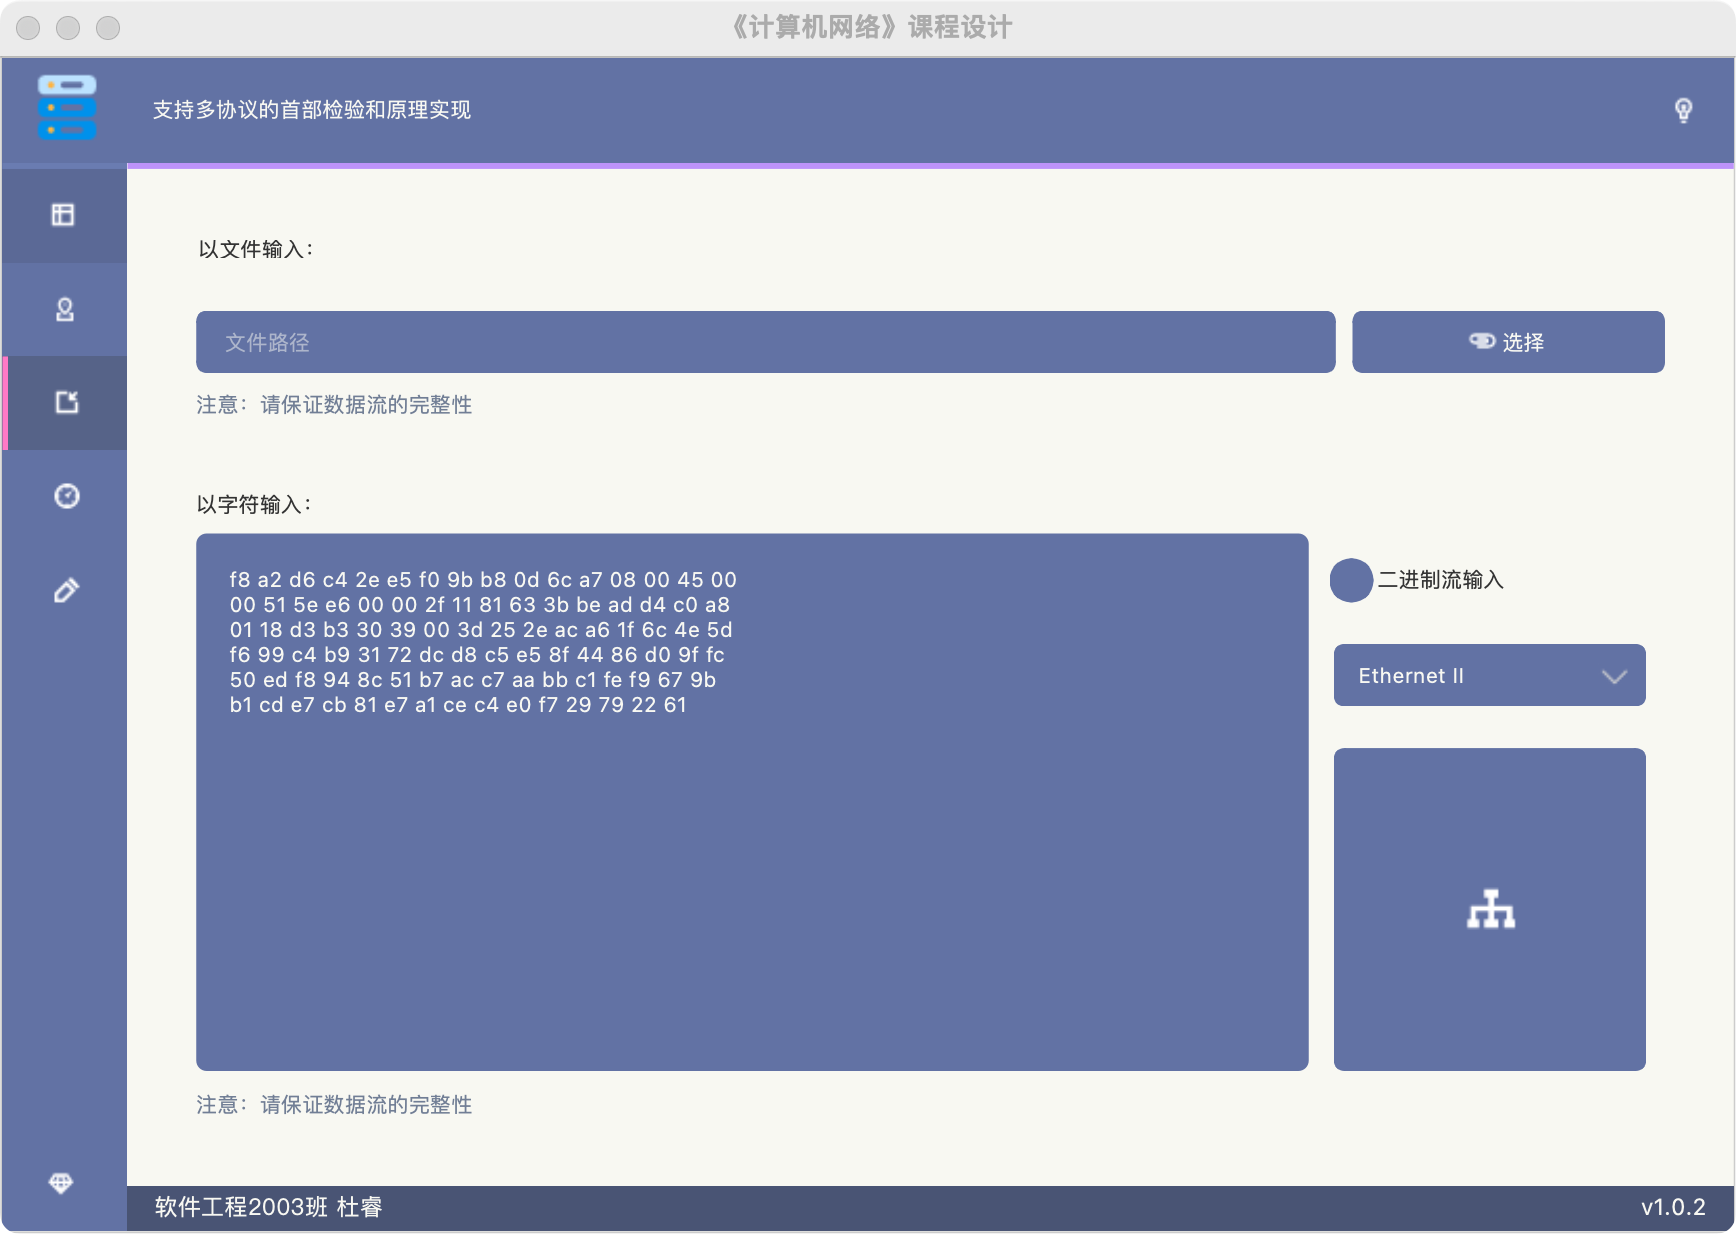
\includegraphics[scale=0.23]{index-input.png}
    \caption{输入}
\end{figure}

\begin{figure}[htbp]
    \centering
    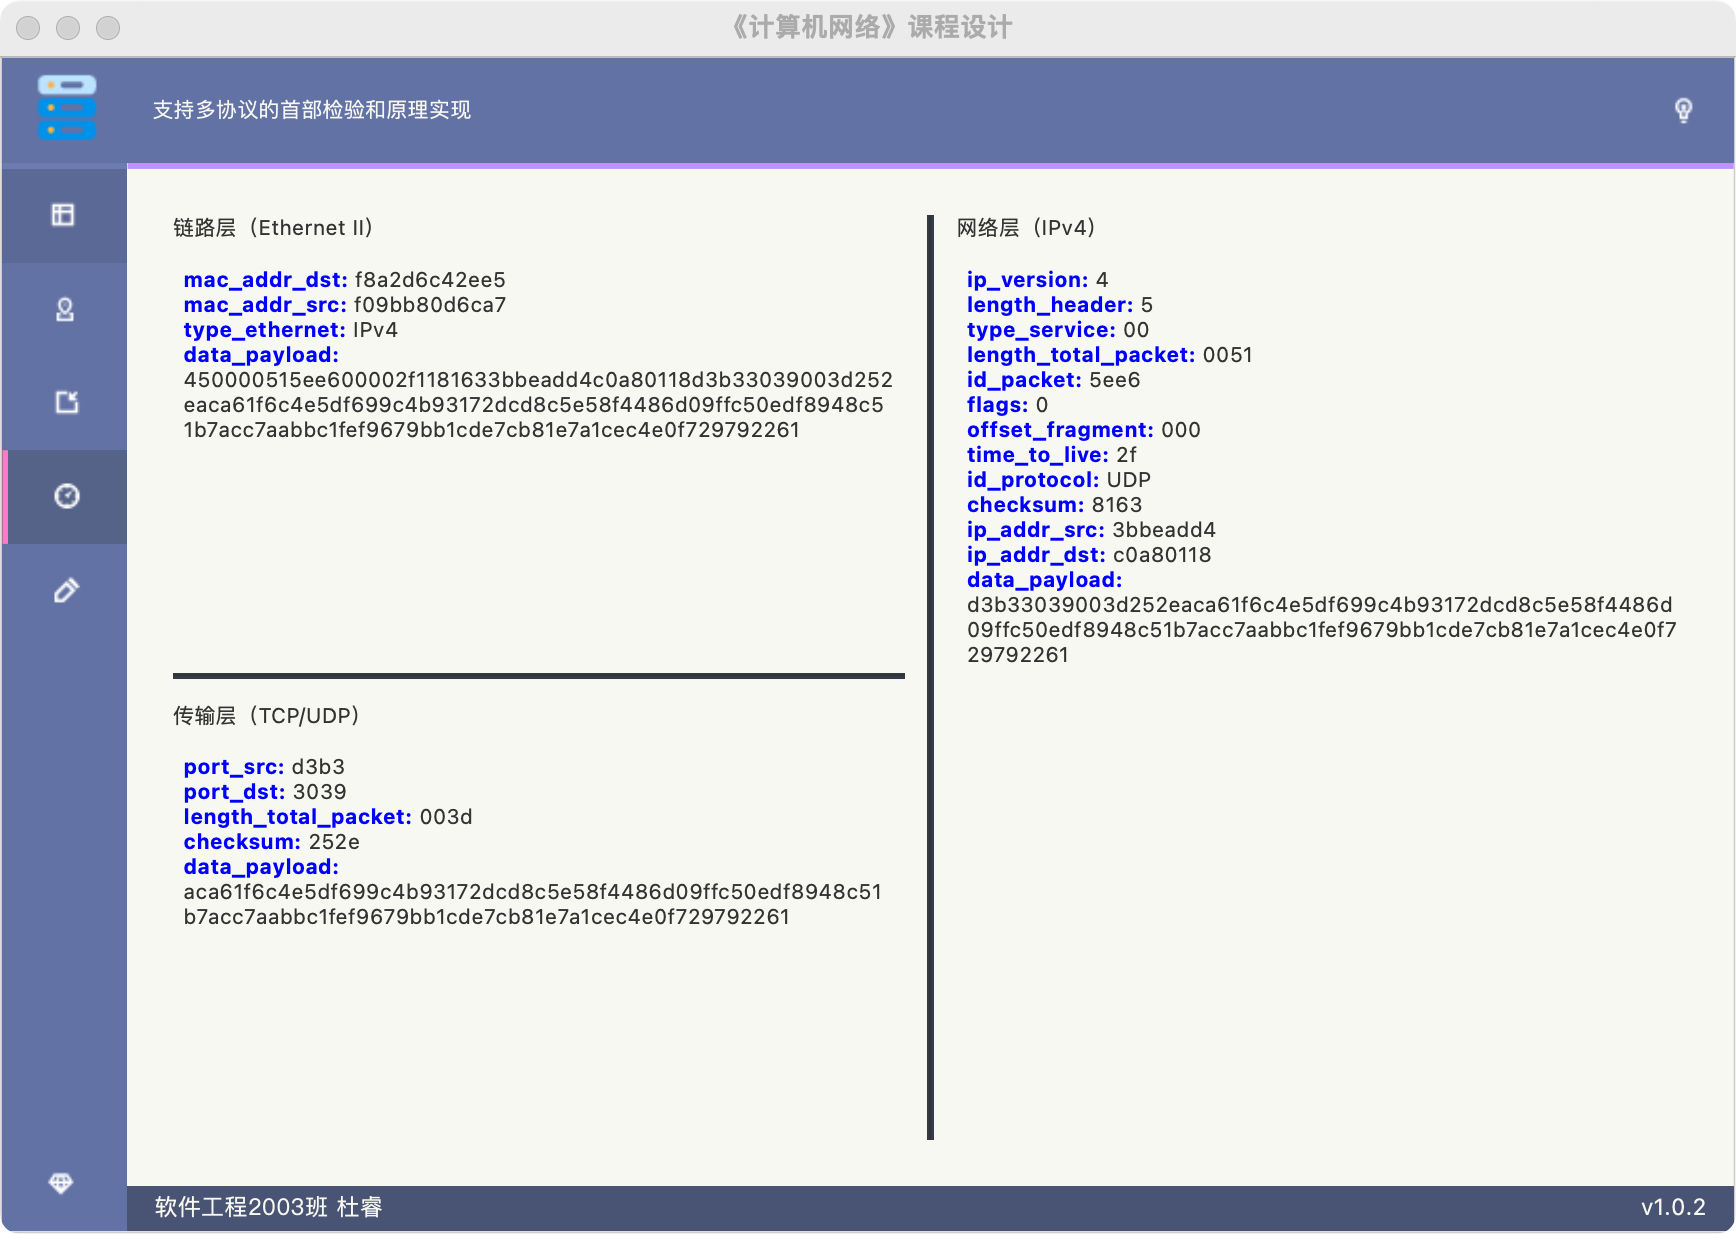
\includegraphics[scale=0.23]{index-par.png}
    \caption{解析}
\end{figure}

\begin{figure}[htbp]
    \centering
    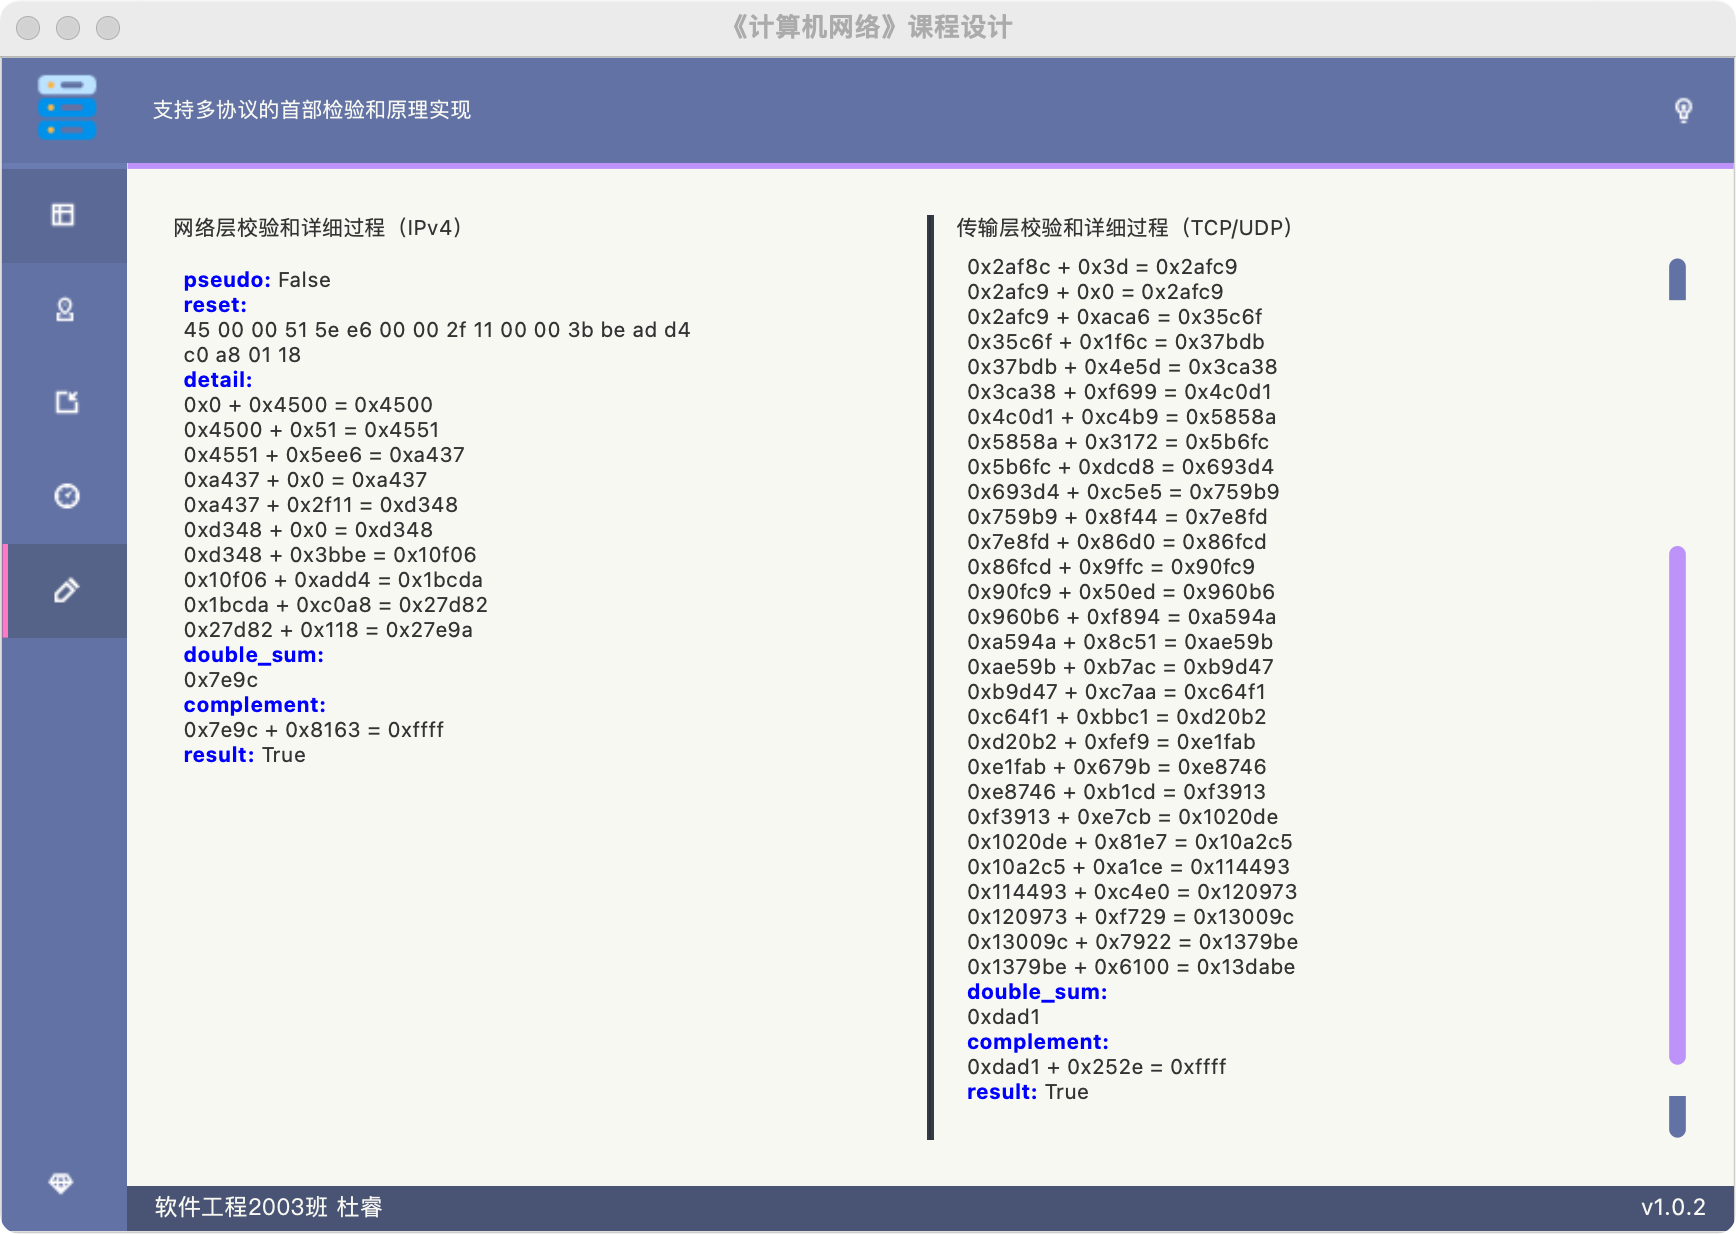
\includegraphics[scale=0.23]{index-calc.png}
    \caption{检验详细过程}
\end{figure}

\subsection{存在问题及思考}

\noindent 校验和计算模块的时间复杂度为O(n),其中n为数据包首部中的字节数。由于数据包首部的字节数通常都比较小,因此也可以认为是常数级别的。问题:

\begin{description}
	\item [已修正] 经过多次实际测试,发现原有程序对于首部含0的数据包存在解析位偏移的情况。原因有:1. 进制转化过程,不会检查长度损失;2. 伪首部长度字段子要考虑补零。
	\item [未修正] 在真实场景中,WireShark对于数据包会有尾部补丁导致伪首部长度计算错误的情况。这是数据链路层负责的部分,因本程序的职责链只考虑了头部和数据部分,故难以修正。
\end{description}



\newpage
\section{课设总结}

肤浅地说,解析无非就是把一长串字符串进行分割解释,校验无非就是做十六进制加法;可是,在实现的过程中,我愈发觉得计算机网络的设计无比奥妙。这种神奇之处,在于实现一个及其复杂的过程(例如两个人之间发送邮件),可以讲职责分拆至各个层次,每一层使用下一层提供的服务,并向上层提供服务。也就是说,我们看到的数据流,虽然看似是线性的,可实则是分层分时构建(解析)的。所以,遵循这一原则,就可以简化并复用代码。本次设计使用WireShark进行抓包,让我对计算机网络的原理有了实践性的认识。程序的健壮性方面,本程序在函数内部引入了断言(Assert)机制,可以很好的返回错误信息,便于调试。此外,学习使用PyQt和Rich库,使我对于UI有了新的认识。

\end{CJK}
\end{spacing}
\end{document}